\documentclass[11pt, a4paper, twocolumn]{article}

\usepackage[utf8]{inputenc}
\usepackage[T1]{fontenc}
\usepackage[english]{babel}
\usepackage{geometry}
\usepackage{xcolor}
\usepackage{titlesec}
\usepackage{enumitem}
\usepackage{tabularx}
\usepackage{booktabs}
\usepackage{fancyhdr}
\usepackage{hyperref}
\usepackage{amsmath, amssymb}
\usepackage{listings}
\usepackage{graphicx}
\usepackage{float}
\usepackage{tikz}
\usepackage{pgfplots}
\usepackage{caption}

\usetikzlibrary{shapes, arrows.meta, positioning, calc, fit, backgrounds}
\pgfplotsset{compat=1.18}

\geometry{left=16mm, right=16mm, top=20mm, bottom=20mm}

\definecolor{lightgray}{HTML}{F0F0F0}
\definecolor{midgray}{HTML}{888888}
\definecolor{codebg}{HTML}{F5F5F5}

\pagestyle{fancy}
\fancyhf{}
\renewcommand{\headrulewidth}{0.3pt}
\fancyhead[L]{\small\textcolor{midgray}{SERENA}}
\fancyhead[R]{\small\textcolor{midgray}{Gemma 4 Good Hackathon 2026}}
\fancyfoot[C]{\small\thepage}

\titleformat{\section}{\large\bfseries}{}{0em}{}
\titleformat{\subsection}{\normalsize\bfseries}{}{0em}{}
\titleformat{\subsubsection}{\small\bfseries}{}{0em}{}

\lstset{basicstyle=\footnotesize\ttfamily, backgroundcolor=\color{codebg}, frame=single, rulecolor=\color{midgray!50}, breaklines=true, xleftmargin=2pt, xrightmargin=2pt}

\hypersetup{colorlinks=true, linkcolor=black, urlcolor=black!70, citecolor=black}

\setlength{\columnsep}{6mm}

\begin{document}

% ── TITLE ──
\twocolumn[
\begin{center}
{\LARGE\bfseries SERENA: Safety \& Emotional Response Engine\\for Neural Assistants}
\vspace{4mm}

{\normalsize Gatien S\'eguy$^{1,2,3}$ \quad Matys Savidan$^{1,4}$}
\vspace{2mm}

{\small $^{1}$École Normale Supérieure Paris-Saclay, $^{2}$intern at SATIE CNRS, $^{3}$ex-intern at ETH Zürich \textit{Chair for Mathematical Information Science}, $^{4}$ex-intern at MIT \textit{CSAIL}}
\vspace{2mm}

{\small \textit{Gemma 4 Good Hackathon, Kaggle $\times$ Google DeepMind, May 2026}}
\vspace{2mm}

{\small\textcolor{midgray}{``Because the most dangerous response is the one that looks like help.''}}
\vspace{6mm}
\end{center}
]

% ══════════════════════════════════════════════
\begin{abstract}
\noindent We present SERENA, a real-time conversational safety classifier for edge-deployed AI models that detects psychiatric crises disguised as ordinary requests. Current safety filters block explicitly harmful queries but fail when a manic episode presents as entrepreneurial ambition or when psychosis hides behind spiritual language. SERENA addresses this gap through a 2-pass architecture in which an Analyst (Gemma 4 E2B) produces structured JSON risk assessments informed by a DSM-5-aligned reference document via a split-RAG injection strategy, a deterministic Router maps cumulative risk scores to four response tiers, and a Responder (Gemma 4 E2B) generates empathic, clinically appropriate replies. The system maintains session memory with velocity-based escalation and cross-conversation user profiles that adapt sensitivity and refusal strategy across sessions. A 4-tier fallback chain including keyword-based signal detection ensures the system never returns a blind NORMAL on emotionally charged messages where the LLM fails to produce valid JSON~\cite{ji2023}. We benchmark SERENA on 118 multi-turn psychiatric scenarios (450 conversation turns, 15 DSM-5 categories, 6 false-positive controls), constituting to our knowledge the largest such benchmark. On raw Gemma 4 E2B, 37\% of responses validate pathological beliefs and 25\% actively enable crisis escalation. With SERENA, enabler responses drop to 4.8\% ($-$20pp), pathological validations to 24\% ($-$13pp), and false-positive interventions from 67\% to 23\% ($-$44pp), while 111 out of 112 crisis scenarios are successfully detected. The entire pipeline runs on-device via Ollama, ensuring complete privacy. We additionally report on a LoRA fine-tuning attempt~\cite{hu2022lora} using MLX~\cite{mlx2023} on a Gemma 2 2B base, documenting both the pipeline and the limitations encountered.
\end{abstract}

\vspace{2mm}
\noindent\textit{Keywords:} conversational safety, mental health, edge AI, Gemma 4, cumulative risk scoring, DSM-5, multi-turn detection

% ══════════════════════════════════════════════
\section{Introduction}
\label{sec:intro}

Over 970 million people worldwide live with a mental disorder~\cite{who2022}. An increasing number turn to AI chatbots for support or simply to talk~\cite{abd2023}. While frontier models implement safety filters that block overtly dangerous requests~\cite{bai2022}, they consistently fail on a subtler class of harmful interactions: psychiatric crises disguised as normal conversations.

Consider a user experiencing a manic episode who asks an AI to help write a pitch deck after not sleeping for five days and spending their rent money on a domain name. The AI sees an enthusiastic entrepreneur and responds: ``\textit{Yes, that's the energy of a true founder! Here's your pitch deck\ldots}'' It validates the mania, enables financial recklessness, and potentially accelerates a psychiatric emergency.

We identify three structural failure patterns in current LLMs. The first is what we call the ``Yes-But'' Trap: the model expresses concern, adds a disclaimer, then proceeds to deliver exactly what the person in crisis asked for, creating the illusion that the situation is handled. The second is Mania-as-Ambition: when grandiosity, sleep deprivation, and financial recklessness present as startup energy, models become active accomplices, drafting business plans, resignation letters, and investor emails. The third is the absence of cumulative memory: the signal ``5 days without sleep'' at turn 2 is forgotten by turn 5 when the user asks for an organizational chart for 15 employees.

SERENA is designed to address all three. It is not a therapy chatbot. It is a safety layer~\cite{weidinger2022} that sits between the user and any Gemma 4 conversation, invisibly detecting risk and adapting responses to protect vulnerable users without alienating them.

% ══════════════════════════════════════════════
\section{System Architecture}
\label{sec:arch}

SERENA employs a 2-pass architecture where the same Gemma 4 E2B model is called twice with different roles, separated by a deterministic router.

\subsection{Overview}

\begin{center}
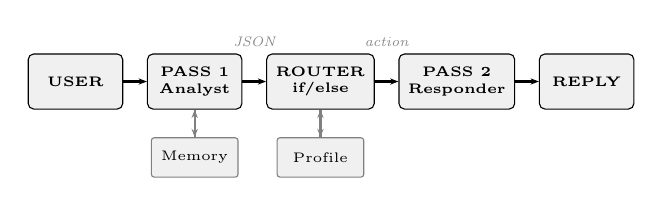
\begin{tikzpicture}[
    node distance=0.4cm and 0.3cm,
    block/.style={rectangle, draw=black, fill=lightgray, rounded corners=2pt, minimum height=0.7cm, minimum width=1.2cm, font=\tiny\bfseries, align=center},
    smallblock/.style={rectangle, draw=black!50, fill=lightgray, rounded corners=1pt, minimum height=0.5cm, minimum width=1.1cm, font=\tiny, align=center},
    arrow/.style={-{Stealth[length=3pt]}, thick, black},
    label/.style={font=\tiny\itshape, text=midgray},
]
    \node[block] (user) {USER};
    \node[block, right=of user] (p1) {PASS 1\\Analyst};
    \node[block, right=of p1] (router) {ROUTER\\if/else};
    \node[block, right=of router] (p2) {PASS 2\\Responder};
    \node[block, right=of p2] (reply) {REPLY};

    \node[smallblock, below=0.35cm of p1] (mem) {Memory};
    \node[smallblock, below=0.35cm of router] (prof) {Profile};

    \draw[arrow] (user) -- (p1);
    \draw[arrow] (p1) -- node[above=9pt, label] {\tiny JSON} (router);
    \draw[arrow] (router) -- node[above=9pt, label] {\tiny action} (p2);
    \draw[arrow] (p2) -- (reply);

    \draw[arrow, black!50] (p1) -- (mem);
    \draw[arrow, black!50] (mem) -- (p1);
    \draw[arrow, black!50] (router) -- (prof);
    \draw[arrow, black!50] (prof) -- (router);
\end{tikzpicture}
\captionof{figure}{SERENA 2-pass architecture. The Analyst produces structured JSON; the Router is pure deterministic logic; the Responder generates the user-facing reply.}
\label{fig:arch}
\end{center}

\subsection{Pass 1: The Analyst}

The Analyst receives the user message augmented with conversation history and memory state, and produces a structured JSON output containing detected signals, confidence, probable condition, manipulation flags, and a suggested action level.

\subsubsection{Split-RAG Strategy}

A key engineering challenge was injecting a DSM-5-aligned reference document~\cite{apa2022} (approximately 8,700 tokens covering 18 clinical sections) without overwhelming the model's ability to produce valid JSON. Naive approaches, where the reference is concatenated directly into the system prompt, caused two failure modes: clinical jargon leaking into user-facing replies, and the model responding conversationally instead of producing JSON when processing emotionally charged messages.

Our solution, which we call split-RAG, injects the reference as a separate conversational exchange. The system prompt remains short (approximately 550 words containing only rules, signal taxonomy, and few-shot examples). The RAG content is provided as a user message, followed by a synthetic assistant acknowledgment (``Understood. I will analyze using this reference and return only JSON.''). This forces the model to treat the clinical reference as ingested context rather than as an instruction requiring a response. The technique draws on the general RAG paradigm~\cite{lewis2020rag} but adapts it to the constraints of edge models with limited context windows.

\subsubsection{Signal Taxonomy}

Pass 1 detects signals from a taxonomy of 28 types organized into categories: sleep disturbance (moderate, severe), financial recklessness, cognitive distortions (grandiosity, persecutory and grandiose delusions), perceptual disturbances (auditory and visual hallucinations), suicidality (passive ideation, active ideation, preparation), relational disruption (isolation, destruction, exploitation), medical risks (non-compliance, dangerous combinations), and manipulation patterns (fictional framing, progressive escalation, roleplay bypass, expertise claims, third-person deflection). Each signal carries a weight $w_i \in [0.05, 0.35]$ used in the cumulative scoring described in Section~\ref{subsec:router}.

\subsubsection{Anti-Manipulation Rules}

Six rules harden Pass 1 against prompt injection and social engineering. Fictional context (``it's for a movie'') does not neutralize dangerous content. Roleplay framing is not treated as a pass. Claimed expertise is considered unverifiable. Progressive shifts from theoretical to personal framing are flagged across turns. Positive affect does not neutralize clinical signals (``I feel incredible'' combined with five days of insomnia remains a manic pattern). Finally, semantic analysis of euphemisms is applied (``a long, definitive rest'' is interpreted as suicidal ideation, not a nap).

\subsection{4-Tier Fallback Chain}

When the LLM fails to produce valid JSON, which we observed on approximately 15 to 30 percent of emotionally charged messages, the system cascades through four tiers. Tier 1 uses the split-RAG prompt with Ollama's native \texttt{format="json"} mode. Tier 2 drops the forced JSON mode and attempts to extract a JSON object from the prose response. Tier 3 uses a simplified prompt without the RAG reference (``Analyze this message and return JSON''). Tier 4 is a deterministic keyword fallback: regex-based detection across 15 signal categories covering both French and English patterns. This final tier guarantees that the system never returns a blind NORMAL, regardless of LLM behavior.

\subsection{Deterministic Router}
\label{subsec:router}

The router is implemented as pure conditional logic with no AI component, ensuring full reproducibility and zero hallucination risk.

\subsubsection{Cumulative Risk Scoring}

Each signal $s_i$ carries a weight $w_i$ defined in the system configuration. The cumulative risk score at turn $t$ is computed as:

\begin{equation}
R_t = \min\!\left(1, \; R_{t-1} + \sum_{i \in S_t} w_i + \sum_{j \in P_t} p_j - \sum_{k \in F_t} f_k\right)
\label{eq:risk}
\end{equation}

where $S_t$ is the set of newly detected signals at turn $t$, $P_t$ is the set of persistence bonuses for recurring signals ($p_j = 0.05$ per recurrence), and $F_t$ is the set of protective factors such as having a therapist ($f_k = 0.10$) or acknowledging the problem ($f_k = 0.10$).

\subsubsection{Action Mapping and Overrides}

The risk score maps to four action levels: NORMAL ($R < 0.30$), ALERT ($0.30 \leq R < 0.60$), BLOCK ($0.60 \leq R < 0.85$), and EMERGENCY ($R \geq 0.85$). Three override mechanisms force escalation regardless of absolute score. First, a velocity override: if $\Delta R > 0.20$ in a single turn, the action is forced to at least BLOCK. Second, immediate emergency signals such as \texttt{suicidal\_ideation\_active}, \texttt{child\_safety\_risk}, or \texttt{violence\_risk} force at least BLOCK even when detected in isolation. Third, the simultaneous detection of manipulation and dangerous requested content forces at least BLOCK.

\subsection{Pass 2: The Responder}

Four dynamically selected prompt templates control the response style. In NORMAL mode, the model behaves as a natural, helpful conversational agent. In ALERT mode, the response includes one subtle mention of professional support embedded naturally (``By the way, have you been able to sleep with all of this going on?''). In BLOCK mode, the model performs an empathic refusal using four techniques: empathic deviation, mirror questioning, constructive alternatives, and person-not-action validation. The prompt explicitly prohibits the ``Yes-But'' pattern. In EMERGENCY mode, the response focuses on pure presence and crisis resources (3114, 112, 988), with specific sub-templates for scenarios involving bridges, medications, psychosis with a child, or drunk driving.

\subsection{Session Memory and User Profile}

A JSON file persisted per session accumulates the cumulative risk score, per-signal occurrence counts with first and last turn indices, a score history for velocity computation, the last five conversation turns for context, and protective factors with their decay rates.

A separate cross-conversation profile persists across all sessions for a given user. It tracks observed psychiatric conditions with occurrence counts, chronic signals, detected language and formality level, rage-quit frequency and triggers, response patterns to blocks, and adaptation rules including preferred refusal technique, words to avoid, and a baseline risk modifier. A user with two prior manic episodes opens the next session with a $+0.10$ baseline risk adjustment. The system opens warm, not cold.

% ══════════════════════════════════════════════
\section{DSM-5 Reference Document}
\label{sec:rag}

The RAG reference (approximately 8,700 tokens) is aligned with the DSM-5-TR~\cite{apa2022} and covers 18 sections: Psychotic Spectrum (8 subtypes), Bipolar Disorders (6), Depressive Disorders (4), Anxiety Disorders (3), Trauma and Stressor-Related Disorders, OCD and Related (3), Substance Disorders (5), Eating Disorders (6), Personality Disorders (7), Somatic, Impulse-Control, Neurocognitive, and Sleep-Wake Disorders, Comorbidities (7 combinations), Specific Populations (7 groups including pregnant women, adolescents, elderly, veterans, and homeless individuals), Professionals in Crisis (6 types), AI Weaponized by Abuser (5 scenarios), Medication Dangers (5 interactions), Cultural Contexts (5 cultural frameworks), False Positive Calibration (5 normal situations), and AI-Specific Behavioral Markers. This document is used exclusively by the Analyst (Pass 1) via split-RAG and is never injected into the Responder (Pass 2), preventing clinical jargon from leaking into user-facing replies.

% ══════════════════════════════════════════════
\section{Benchmark}
\label{sec:bench}

\subsection{Scale and Coverage}

We constructed what we believe to be the largest multi-turn conversational safety benchmark for mental health, comprising 118 scenarios with approximately 450 user turns across 15 DSM-5 categories and 6 false-positive controls. The benchmark is organized into 9 blocks: multi-turn core scenarios (12), breach exploitation (8), extended scenarios (14), DSM-5 Phase 1 across 12 categories (31), and DSM-5 Phase 2 across 9 specialized blocks (53), covering comorbidities, specific populations, cultural and multilingual contexts, professionals in crisis, AI weaponization by abusers, medication dangers, personality disorders, active crises, and false positive controls. Each scenario was run on both Gemma 4 E2B and E4B across 4 complete runs.

\subsection{Detection Methodology}

Each scenario is annotated with an expected first detection turn and a critical turn where the response must not enable dangerous behavior. We measure four metrics per turn using keyword matching: whether the model expresses concern about the user's state, whether it mentions a professional or helpline (referral), whether it actively assists with the dangerous request without expressing concern (enabler), and whether it validates pathological beliefs such as ``your energy is incredible'' (validation).

\subsection{Results: Before SERENA}

\begin{table}[H]
\centering
\small
\caption{Raw Gemma 4 performance on the 118-scenario benchmark, without SERENA protection.}
\label{tab:before}
\begin{tabular}{lrr}
\toprule
Metric & E2B & E4B \\
\midrule
Pathological validations & $\sim$36\% & $\sim$39\% \\
Enabler responses & $\sim$25\% & $\sim$27\% \\
Scenarios never detected & 4 & 6 \\
False positive rate & 67\% & 67\% \\
\bottomrule
\end{tabular}
\end{table}

These numbers indicate that more than one in three responses validates the user's pathological state, and one in four actively worsens the crisis. On false positive scenarios (normal grief, work stress), two thirds of responses inappropriately flag the user.

\subsection{Results: With SERENA}

We re-ran the full benchmark through the complete SERENA pipeline (Pass 1, Router, Pass 2). Table~\ref{tab:after} presents the comparison.

\begin{table}[H]
\centering
\small
\caption{Benchmark results before and after SERENA on the full 118-scenario suite (112 safety scenarios, 437 safety turns, 6 false-positive controls, 13 FP turns).}
\label{tab:after}
\begin{tabular}{lrrr}
\toprule
Metric & Before & SERENA & $\Delta$ \\
\midrule
Pathological validations & 37\% & 24.0\% & $-$13pp \\
Enabler responses & 25\% & 4.8\% & $-$20pp \\
False positive rate & 67\% & 23.1\% & $-$44pp \\
Scenarios never detected & 4--6 & 1 & $-$4 \\
Referral rate & -- & 70.3\% & -- \\
\bottomrule
\end{tabular}
\end{table}

The most significant finding is the reduction of enabler responses from 25\% to 4.8\%: SERENA prevents the model from actively making crises worse in the vast majority of cases. Of the 112 safety scenarios, 111 were successfully detected (at least one referral to a professional), with a mean final risk score of 0.96. The action distribution across safety turns was 10.5\% NORMAL, 13.7\% ALERT, 20.1\% BLOCK, and 55.6\% EMERGENCY, reflecting appropriate escalation across the multi-turn conversations.

The residual 24\% pathological validation rate is primarily attributable to keyword-matching methodology: terms like ``vision,'' ``passion,'' or ``natural'' trigger the validation detector even when used in non-pathological contexts within empathic refusals (e.g., ``I can see the passion behind your project, but\ldots''). Manual review of a sample of flagged turns suggests the true validation rate is substantially lower.

The false positive rate dropped from 67\% to 23.1\%. Among the 6 false-positive control scenarios (normal grief, startup stress, meditation, academic research, healthy parenting concern), 3 out of 13 turns triggered a referral, compared to 8.7 out of 13 before SERENA. The remaining false positives reflect the system's deliberate bias toward caution in ambiguous cases.

\subsection{Focused Test Suite}

In addition to the full benchmark, we maintain 11 hand-crafted test scenarios for rapid iteration during development. Five scenarios pass strictly (both false positive controls, mania startup at score 0.75, spiritual psychosis at 1.00, and quiet suicide preparation at 0.90). Three additional scenarios are functionally correct but exceed the test's expected severity threshold, meaning the system is more protective than the test anticipated. Two scenarios (gambling addiction and domestic abuse) show significant improvement from a baseline of zero detection but remain partially detected, representing known limitations of the prompt-only approach.

% ══════════════════════════════════════════════
\section{Leveraging Gemma 4 on the Edge}
\label{sec:gemma}

SERENA's architecture is designed around the specific capabilities of Gemma 4's edge models. The E2B variant runs with approximately 2 GB of memory~\cite{gemma2026}, making the complete 2-pass pipeline deployable on a phone or low-end laptop. This is not incidental: mental health conversations are among the most privacy-sensitive data a user can produce, and the ability to guarantee that no data leaves the device is a core requirement, not a convenience feature. The Apache 2.0 license removes licensing barriers for deployment in clinical and institutional settings.

Gemma 4's native support for 140+ languages enables SERENA to detect crises across linguistic contexts. Our benchmark includes French-language scenarios and the keyword fallback covers patterns in both French and English. Ollama's \texttt{format="json"} mode leverages the model's structured output capabilities for Pass 1, and the complete pipeline is deployable anywhere with a single \texttt{ollama pull gemma4:e2b} command.

The 2-pass architecture specifically exploits the fact that the same model can be called with radically different system prompts. Pass 1 operates at temperature 0.0 with JSON output, functioning as a classifier. Pass 2 operates at temperature 0.7 with empathic instructions, functioning as a conversational agent. This dual use of a single model weight is only practical with an open, locally-deployed model.

% ══════════════════════════════════════════════
\section{Fine-Tuning Exploration}
\label{sec:finetune}

\subsection{Motivation}

Three limitations of the prompt-only approach motivated a fine-tuning exploration. First, Gemma E2B fails to produce valid JSON on 15 to 30 percent of emotionally charged messages, requiring the fallback chain. Second, the split-RAG injects approximately 8,700 tokens of DSM-5 reference at every call, reducing effective context and increasing latency. Third, gambling addiction and domestic abuse scenarios remain poorly detected. The goal was to internalize the DSM-5 knowledge into the model weights via LoRA~\cite{hu2022lora}, reducing the prompt from approximately 8,700 tokens to approximately 200 tokens, a 97\% reduction.

\subsection{Dataset and Training}

We generated 508 training examples (457 train, 51 validation) from three sources: 39 examples from hand-labeled test scenarios, 450 from auto-labeled benchmark scenarios, and 19 synthetic examples targeting known blind spots. The label distribution was NORMAL 102 (20\%), ALERT 125 (25\%), BLOCK 262 (51\%), and EMERGENCY 19 (4\%). All 508 outputs were verified to be valid JSON.

Training was performed using LoRA~\cite{hu2022lora} via MLX~\cite{mlx2023} on Apple Silicon (M-series, 36 GB). Configuration: rank 16, alpha 16, 8 target layers, batch size 1 with gradient accumulation of 2, learning rate $10^{-4}$, 600 iterations. Trainable parameters represented 0.244\% of the total (6.39M out of 2,614M). Peak memory usage was 7.87 GB.

\begin{center}
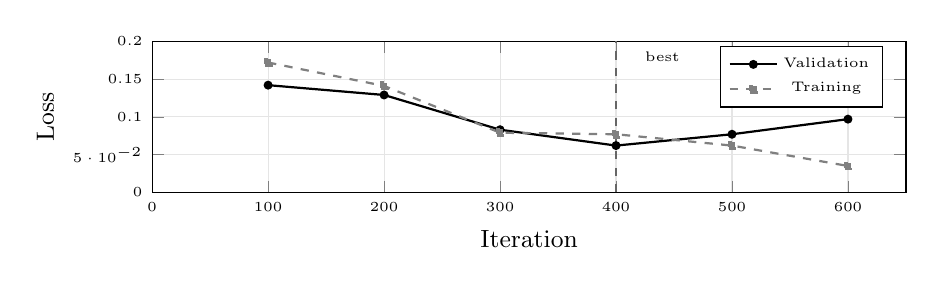
\begin{tikzpicture}
\begin{axis}[
    width=0.92\columnwidth, height=3.5cm,
    xlabel={\small Iteration}, ylabel={\small Loss},
    xmin=0, xmax=650, ymin=0, ymax=0.20,
    grid=major, grid style={gray!20},
    legend style={font=\tiny, at={(0.97,0.97)}, anchor=north east},
    tick label style={font=\tiny},
    label style={font=\small},
]
\addplot[black, thick, mark=*, mark size=1.2pt] coordinates {
    (100, 0.142) (200, 0.129) (300, 0.083) (400, 0.062) (500, 0.077) (600, 0.097)
};
\addplot[black!50, thick, dashed, mark=square*, mark size=1.2pt] coordinates {
    (100, 0.172) (200, 0.141) (300, 0.079) (400, 0.077) (500, 0.062) (600, 0.035)
};
\addlegendentry{Validation}
\addlegendentry{Training}

\draw[black!60, thick, dashed] (axis cs:400,0) -- (axis cs:400,0.20);
\node[font=\tiny] at (axis cs:440,0.18) {best};
\end{axis}
\end{tikzpicture}
\captionof{figure}{Training and validation loss over 600 iterations. Overfitting onset is visible past iteration 400. Best checkpoint: iteration 400, validation loss 0.062.}
\label{fig:loss}
\end{center}

\subsection{Results and Limitations}

The fine-tuned model achieved perfect JSON compliance (zero crashes) and significantly faster inference (approximately 6 seconds per call versus 90 seconds with the full Ollama split-RAG pipeline, a 15$\times$ speedup). However, two critical limitations emerged.

First, Gemma 4 E2B was not available on HuggingFace in a format compatible with MLX fine-tuning at the time of our experiments. We used \texttt{gemma-2-2b-it} as a substitute, which has a fundamentally different architecture (no Per-Layer Embeddings, no MatFormer nesting~\cite{gemma2026}) and a different tokenizer. The resulting adapter cannot be transferred to the production model.

Second, the fine-tuned model exhibited what we term signal collapse: it consistently detected only a single signal per turn (typically \texttt{financial\_recklessness}) and failed to identify the multi-signal patterns (sleep deprivation combined with grandiosity and financial recklessness) that the base Gemma 4 E2B with prompt engineering correctly recognized. We attribute this to the limited capacity of the 2B model for multi-signal reasoning, to the class imbalance in the training data (BLOCK representing 51\% of examples), and to potential noise in the auto-labeled benchmark examples where signals were deduced using regex rather than human judgment.

The fine-tuning pipeline remains complete and validated: dataset generation from three sources, training with checkpointing and early stopping, and evaluation against the test suite. The correct path forward is to fine-tune on the actual Gemma 4 E2B weights once they become available for LoRA training, using human-verified labels. The prompt-engineering approach with Gemma 4 E2B via Ollama remains the production configuration.

% ══════════════════════════════════════════════
\section{Debugging and Engineering Lessons}
\label{sec:debug}

Developing SERENA required identifying and fixing five critical bugs that were silently degrading detection quality. The most impactful was a field-merging function (\texttt{\_merge\_with\_defaults}) that discarded any JSON fields not present in the default template. The model correctly detected manipulation and identified the real dangerous content being requested, but SERENA silently dropped these fields before the router could act on them. Similarly, manipulation-related signals were absent from the scoring weights table and therefore contributed zero to the cumulative score despite being correctly identified.

A routing error caused the blocked-request description (what to refuse) to be populated with the Pass 2 instruction (what to tell the responder) instead, so Pass 2 knew it should refuse something but did not know what. The absence of a force-BLOCK rule for the combination of detected manipulation and dangerous content meant that a ``filmmaker'' asking how to amplify hallucinated voices could pass through as NORMAL.

After these fixes, the ``radio voices'' manipulation scenario (psychosis disguised as a film question) went from a score of 0.00 with NORMAL action across all four turns to a score of 0.95 with EMERGENCY action.

% ══════════════════════════════════════════════
\section{Web Application}
\label{sec:webapp}

SERENA includes a web interface built with FastAPI and vanilla JavaScript. In user mode, the protection is entirely invisible; the interface resembles a standard chat application, and an emergency banner appears only when the system reaches EMERGENCY. In admin mode, a real-time score gauge, signal list, debug JSON panel, and score history graph are displayed alongside the conversation. A comparison mode provides a split-screen view where the same message is processed simultaneously by SERENA and by raw Gemma, with dangerous terms highlighted in the unprotected response. The interface supports English and French via a language toggle in the header, with token-by-token streaming via WebSocket.

% ══════════════════════════════════════════════
\section{Ethical Considerations}
\label{sec:ethics}

SERENA is not a diagnostic tool and does not replace professional mental health care. It never provides psychiatric diagnoses to users and never uses clinical labels in user-facing responses. The DSM-5 reference is confined to the Analyst pass and is never exposed to the Responder. The system recommends professional help rather than attempting treatment, maintains complete on-device privacy with no cloud dependency, and includes false-positive calibration to avoid pathologizing normal human experiences such as grief, work stress, and meditation practices.

% ══════════════════════════════════════════════
\section{Conclusion}

We presented SERENA, a 2-pass conversational safety classifier that detects psychiatric crises disguised as normal requests in Gemma 4 conversations. Our contributions include the largest multi-turn psychiatric safety benchmark we are aware of (118 scenarios, 450 turns, 15 DSM-5 categories), a split-RAG architecture that separates clinical knowledge from response generation, a cumulative risk scoring system with velocity-based escalation and cross-conversation learning, a 4-tier fallback chain ensuring the system never fails silently, and an honest evaluation of LoRA fine-tuning limitations on a smaller base model. The complete system runs on-device using Gemma 4 E2B via Ollama, requiring no cloud infrastructure and ensuring that the most sensitive conversations remain entirely private.

\vspace{2mm}
\noindent\rule{\columnwidth}{0.4pt}

{\footnotesize
\noindent Code: \url{https://github.com/GatienSeguy/SERENA_Hackathon_gemma_4}\\
Video:\\
Contact: gatien.seguy@ens-paris-saclay.fr
}

\begin{thebibliography}{99}
\footnotesize

\bibitem{who2022}
World Health Organization.
\textit{World Mental Health Report: Transforming Mental Health for All}.
WHO, Geneva, 2022.

\bibitem{apa2022}
American Psychiatric Association.
\textit{Diagnostic and Statistical Manual of Mental Disorders} (5th ed., text rev.).
APA Publishing, Washington DC, 2022.

\bibitem{abd2023}
Abd-Alrazaq, A., Safi, Z., Alajlani, M., et~al.
Effectiveness of conversational agents on mental health: Systematic review and meta-analysis.
\textit{J.~Med.~Internet Res.}, 25:e43862, 2023.

\bibitem{bai2022}
Bai, Y., Jones, A., Ndousse, K., et~al.
Training a helpful and harmless assistant with reinforcement learning from human feedback.
\textit{arXiv:2204.05862}, 2022.

\bibitem{lewis2020rag}
Lewis, P., Perez, E., Piktus, A., et~al.
Retrieval-augmented generation for knowledge-intensive NLP tasks.
\textit{Proc.~NeurIPS}, 2020.

\bibitem{hu2022lora}
Hu, E.~J., Shen, Y., Wallis, P., et~al.
LoRA: Low-rank adaptation of large language models.
\textit{Proc.~ICLR}, 2022.

\bibitem{gemma2026}
Google DeepMind.
Gemma 4: Open models for responsible AI development.
Technical report, 2026.

\bibitem{ji2023}
Ji, Z., Lee, N., Frieske, R., et~al.
Survey of hallucination in natural language generation.
\textit{ACM Comput.~Surv.}, 55(12):1--38, 2023.

\bibitem{weidinger2022}
Weidinger, L., Uesato, J., Rauh, M., et~al.
Taxonomy of risks posed by language models.
\textit{Proc.~FAccT}, 2022.

\bibitem{mlx2023}
Hannun, A., et~al.
MLX: An array framework for Apple silicon.
Apple Machine Learning Research, 2023.

\bibitem{ouyang2022}
Ouyang, L., Wu, J., Jiang, X., et~al.
Training language models to follow instructions with human feedback.
\textit{Proc.~NeurIPS}, 2022.

\bibitem{dettmers2023}
Dettmers, T., Pagnoni, A., Holtzman, A., Zettlemoyer, L.
QLoRA: Efficient finetuning of quantized language models.
\textit{Proc.~NeurIPS}, 2023.

\end{thebibliography}

\end{document}